\documentclass[12pt]{article}
\usepackage[utf8]{inputenc}
\usepackage[spanish]{babel}
\usepackage{amsmath}
\usepackage{amsthm}
\usepackage{graphicx}
\DeclareGraphicsExtensions{.pdf,.png,.jpg}
\usepackage{anyfontsize}
\usepackage{anysize}
\usepackage{tikz}
\usepackage{float}
\usetikzlibrary{patterns}
\usetikzlibrary{calc}
\usetikzlibrary{decorations.markings}
\usetikzlibrary{matrix}
\usepackage{xy}
\usepackage{siunitx}
\usepackage[american,cuteinductors,smartlabels]{circuitikz}
\usetikzlibrary{calc}
\usepackage{color}
\usepackage{listings}
\lstset{ %
language=Python,                % choose the language of the code
basicstyle=\small,       % the size of the fonts that are used for the code
numbers=left,                   % where to put the line-numbers
numberstyle=\small,      % the size of the fonts that are used for the line-numbers
stepnumber=1,                   % the step between two line-numbers. If it is 1 each line will be numbered
numbersep=5pt,                  % how far the line-numbers are from the code
backgroundcolor=\color{white},  % choose the background color. You must add \usepackage{color}
showspaces=false,               % show spaces adding particular underscores
showstringspaces=false,         % underline spaces within strings
showtabs=false,                 % show tabs within strings adding particular underscores
frame=single,   		% adds a frame around the code
tabsize=2,  		% sets default tabsize to 2 spaces
captionpos=b,   		% sets the caption-position to bottom
breaklines=true,    	% sets automatic line breaking
breakatwhitespace=false,    % sets if automatic breaks should only happen at whitespace
escapeinside={\%}          % if you want to add a comment within your code
}
\marginsize{1.5cm}{1.5cm}{0cm}{1.5cm}
\author{M. en C. Gustavo Contreras Mayén.}
\title{Ejercicios EDP Hipérbolicas \\ Curso Física Computacional}
\date{ }
\begin{document}
\maketitle
\fontsize{14}{14}\selectfont
\section*{Para crear una malla circular.}
La solución al problema de la ecuación de Poisson en coordenas polares, requiere un espacio de trabajo precisamente en estas coordenadas, las mallas que hemos usado anteriormente, están diseñadas en coordenadas cartesianas, por lo que para aplicar el algoritmo, necesitamos primero, preparar la malla.
\\
\\
Una manera de hacer esa malla circular, es con el siguiente código:
\begin{lstlisting}
from numpy import *
import matplotlib.pylab as pp

r_a = 0.50
r_b = 1
circulos = 6  
lineas  = 20
origen = (0, 0)

for r in linspace(r_a, r_b, circulos):
    pp.gca().add_patch(pp.Circle(origen, radius=r, fill=False, color='black'))

r_ab = array([r_a, r_b])

for theta in linspace(0, 2 * pi, lineas):
    pp.plot(cos(theta) * r_ab, sin(theta) * r_ab, color='red')

pp.axis('scaled')
pp.title('Creando una malla en coordenadas polares')
pp.show()
\end{lstlisting}
Que nos crea la siguiente figura:
\begin{figure}[H]
\begin{center}
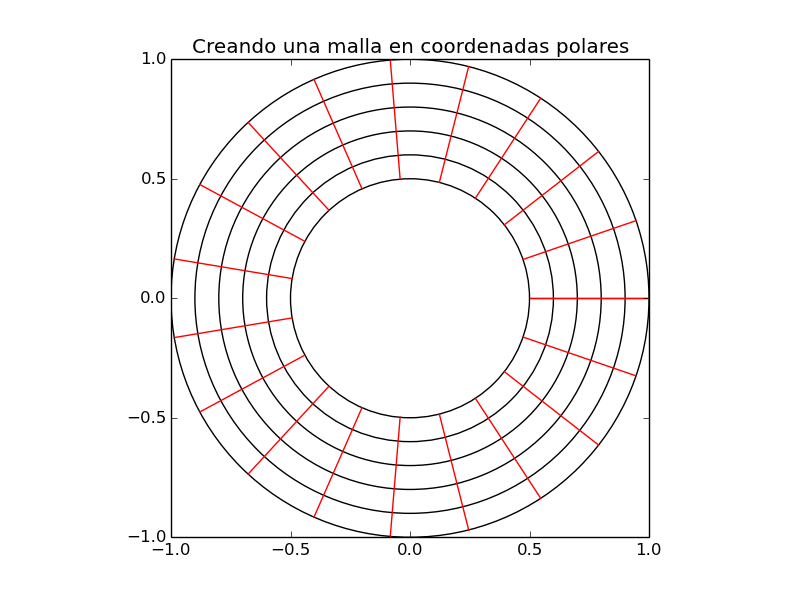
\includegraphics[scale=0.75]{Malla_Circular01.png} 
\caption{Malla circular usando el primer código}
\end{center}
\end{figure}
Otra manera de generar una malla circular, es haciendo algunos ajustes en el código, usando las respectivas reglas de cambio de coordenadas rectangulares a polares.
\begin{lstlisting}
from numpy import *
import matplotlib.pylab as pp

r_a = 0.50
r_b = 1
circulos = 6  
lineas  = 30
origen = (0, 0)

r, t   = meshgrid(linspace(r_a, r_b, circulos), linspace(0, 2 * pi, lineas))
x = r * cos(t)
y = r * sin(t)

pp.plot(x, y)

pp.plot(vstack((x[:,0], x[:, -1])),vstack((y[:,0], y[:, -1])))
           
pp.axis('scaled')
pp.title('Otra manera de generar una malla circular')
pp.show()
\end{lstlisting}
\newpage
El algoritmo anterior nos genera la siguiente gráfica:
\begin{figure}[H]
\begin{center}
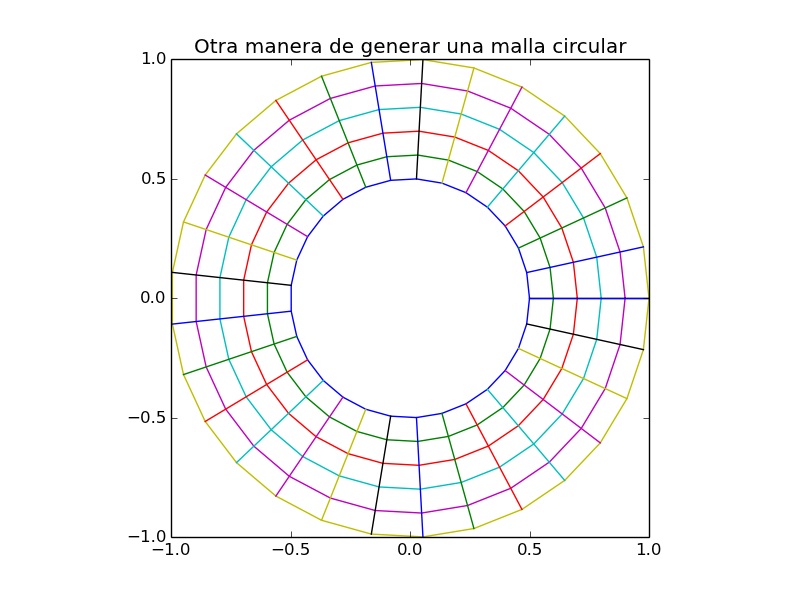
\includegraphics[scale=0.75]{Malla_Circular02.png} 
\caption{Malla circular usando el segundo código}
\end{center}
\end{figure}
Una vez que ya tienen el espacio físico de la malla circular, lo que resta es aplicar el algoritmo por diferencias finitas que debieron de haber desarrollado a partir de la ecuación de Poisson, como se muestra en la figura (2), hay que considerar la distribución de los puntos para ocuparlos en su algoritmo.
\begin{figure}[H]
\begin{center}
\begin{tikzpicture}[font=\small]
	%\tkzDefPoint(0,0){O}
	%\tkzDefPoint(0,5){A}
	\draw (0,0) -- (10,0);
	\draw (5,0) -- (5,5);
	\draw (5,0) -- (2.5,5);
	\draw (5,0) -- (7.5,5);
	\draw [red](10,0) arc[radius=5, start angle=0, end angle=180];
	\draw [red](9,0) arc[radius=4, start angle=0, end angle=180];
	\draw [red](8,0) arc[radius=3, start angle=0, end angle=180];
	\draw [red](7,0) arc[radius=2, start angle=0, end angle=180];
	\draw [fill=black](5,2) circle (0.05) node[above=0.3]{$i-1,j$};
	\draw [fill=black](5,3) circle (0.05) node[above=0.3]{$i,j$};;
	\draw [fill=black](5,4) circle (0.05) node[above=0.3]{$i+1,j$};
	\draw [fill=black](3.65,2.7) circle (0.05) node[left=0.3]{$i,j-1$};
	\draw [fill=black](6.35,2.7) circle (0.05) node[right=0.3]{$i,j+1$};
	%\tkzDrawArc (O,A)(180)
\end{tikzpicture}
\end{center}
\caption{Notación de los índices en coordenadas polares.}
\label{fig:mediocirculo}
\end{figure}
\end{document}